\subsubsection{Quantitative impact of architectural decisions}

Architectural choices directly influence several software qualities (e.g., scalability, reliability, availability, usability).

\highspace
To cope with this, we need metrics to quantify qualities and specific methodologies to analyze the quantitative impact of architectural choices on these qualities. The tactics are also foundational to address the issues.

\highspace
First, before discussing \emph{how to evaluate the quantitative impact of architectural decisions}, we must introduce the availability concept and explain a system life-cycle to introduce some exciting metrics.

\begin{flushleft}
    \textcolor{Green3}{\faIcon{question-circle} \textbf{Why is availability so important?}}
\end{flushleft}
In general, a \textbf{service shall be continuously available} to the user, and if it fails after a bit of downtime, it should be a \textbf{rapid service recovery}. So the \definition{availability} of a service depends on:
\begin{itemize}
    \item The \textbf{complexity} of the \textbf{infrastructure} architecture.
    
    \item \textbf{Reliability} of the individual components.
    
    \item \textbf{Ability to respond} quickly and effectively to faults.

    \item \textbf{Quality of the maintenance} by support organizations and suppliers.

    \item \textbf{Quality} and scope of the \textbf{operational management} processes.
\end{itemize}

\begin{flushleft}
    \textcolor{Green3}{\faIcon{book} \textbf{Study the System Life-Cycle to use availability metrics}}
\end{flushleft}
The \definition{System Life-Cycle} relates to failures in the following way:

\begin{figure}[!htp]
    \centering
    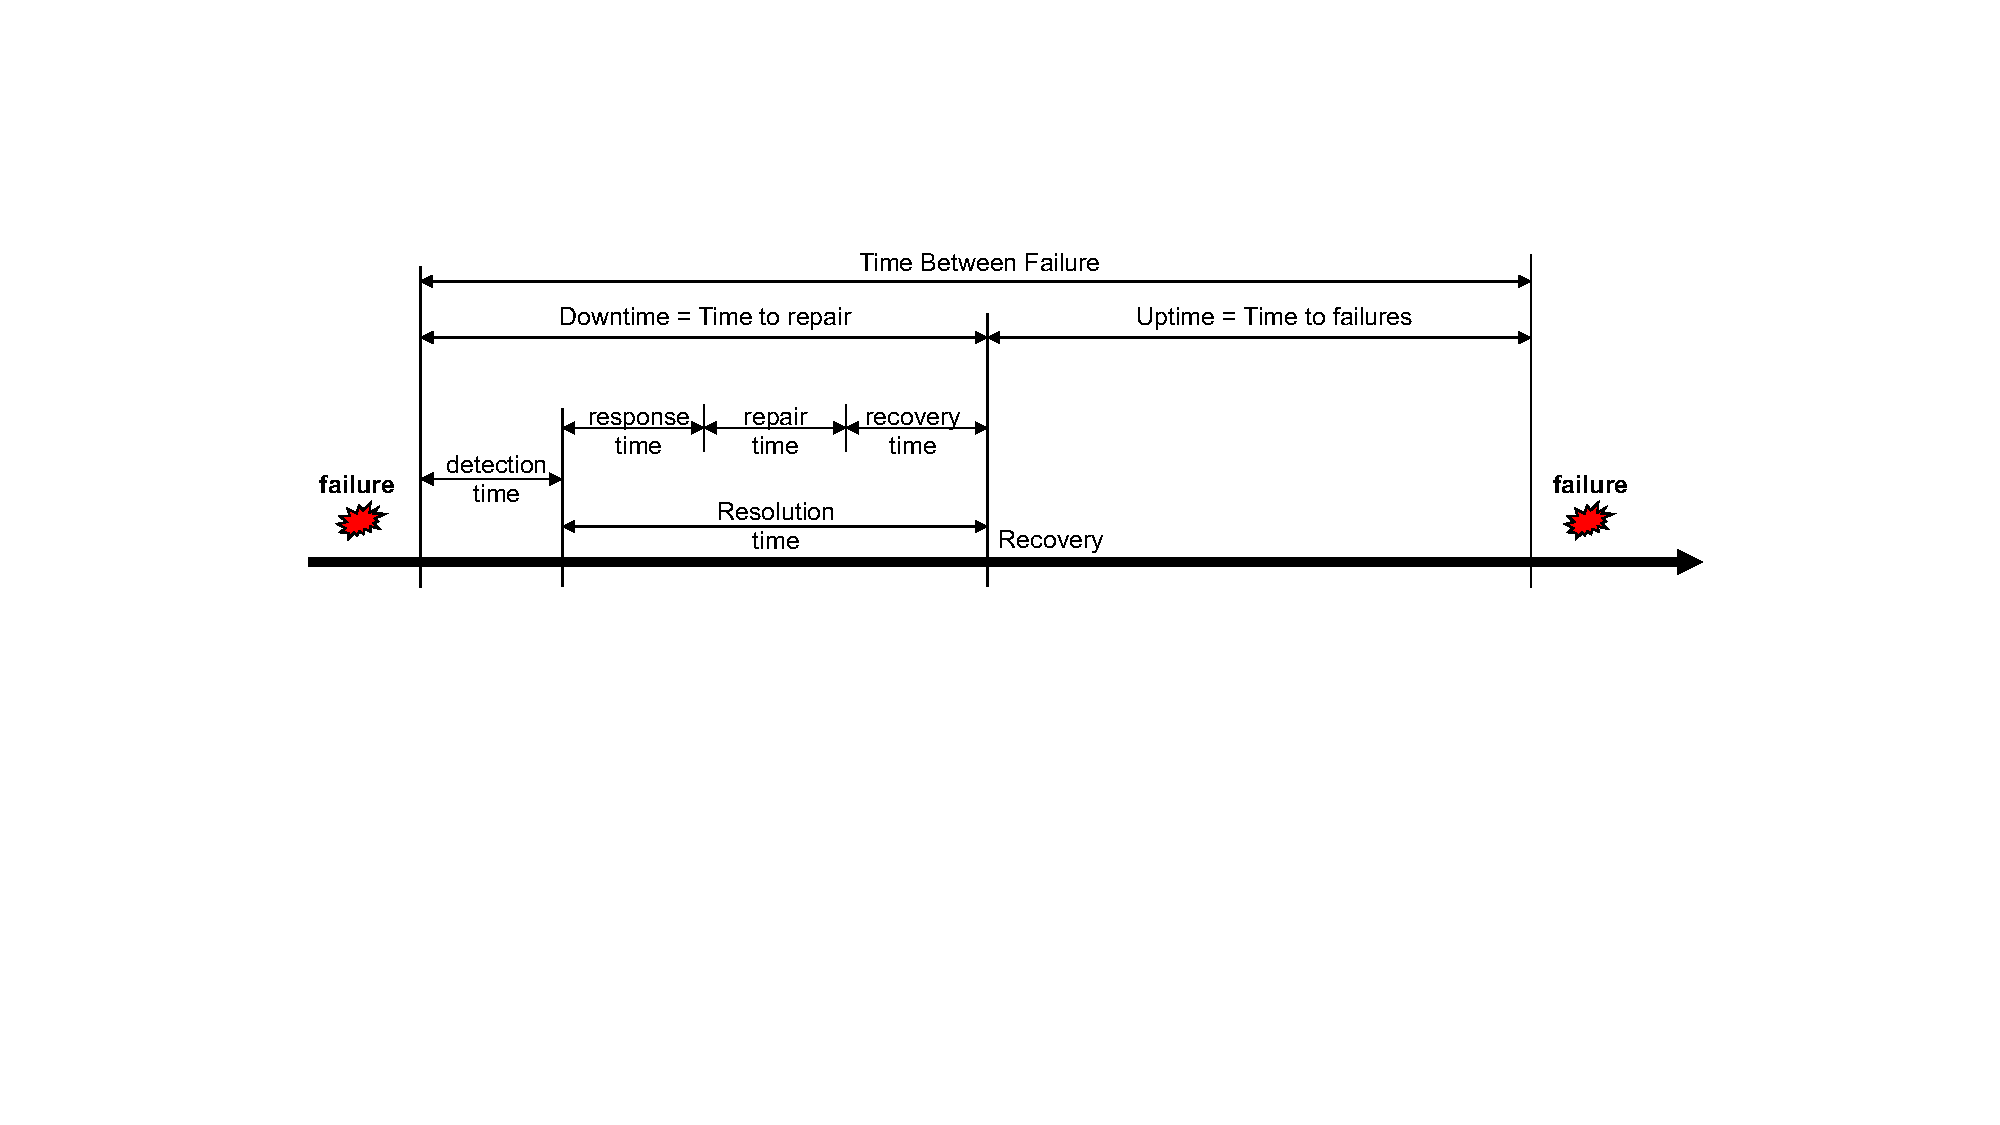
\includegraphics[width=\textwidth]{img/system-life-cycle-1.pdf}
    \caption{The System Life-Cycle when faults occur.}
    \label{fig: The System Life-Cycle when faults occur}
\end{figure}
\begin{itemize}
    \item \textbf{Time of occurrence}. Time at which the \emph{user} becomes aware of the failure.
    
    \item \textbf{Detection time}. Time at which \emph{operators} become aware of the failure.
    
    \item \textbf{Response time}. Time required by \emph{operators} to diagnose the issue and respond to users.
    
    \item \textbf{Repair time}. Time required to fix the service/components that caused the failure.
    
    \item \textbf{Recovery time}. Time required to restore the system (re-configuration, re-initialization, ...).
    
    \item \definition{Mean Time to Repair (MTTR)}. Average time between the occurrence of a failure and service recovery, also known as the \emph{downtime}.

    \item \definition{Mean Time to Failures (MTTF)}. Mean time between the recovery from one failure and the occurrence of the next failure, also known as \emph{uptime}.

    \item \definition{Mean Time Between Failures (MTBF)}. Mean time between the occurrences of two consecutive failures.
\end{itemize}

\begin{definitionbox}[: Availability Metric]
    The \definition{availability metric} is the \textbf{probability} that a \textbf{component} \textbf{works correctly} at \textbf{time} $t$. As a mathematician term, we can express this definition as the relationship between the Mean Time to Failures (MTTF) and the MTTF plus the Mean Time to Repair (MTTR):
    \begin{equation}\label{eq: availability metric}
        A = \dfrac{
            \texttt{MTTF}
        }{
            \texttt{MTTF} + \texttt{MTTR}
        }
    \end{equation}
\end{definitionbox}

\noindent
Note that if the Mean Time to Repair (MTTR) is small, then the Mean Time Between Failures (MTBF) is approximately equal to the Mean Time to Failures (MTTF): $\texttt{MTBF} \approxeq \texttt{MTTF}$.

\begin{flushleft}
    \textcolor{Green3}{\faIcon{question-circle} \textbf{Does an easier notation than the availability metric work?}}
\end{flushleft}
The availability metric is crucial for understanding how a component works at a particular time, but sometimes, we need an easier notation to represent availability. In these cases, we use the \definition{nines notation}.

\highspace
\textbf{Nines} are an informal logarithmic notation for proportions very near to one or, equivalently, percentages very near 100\%. Nines are the number of consecutive nines in a percentage such as 99\% (two nines). The number of nines of a proportion $x$ is:
\begin{equation}\label{eq: nines}
    \texttt{nines} = - \log_{10} \left(1-x\right)
\end{equation}
In the computer system availability (our context), a \emph{one nine} (90\%) uptime indicates a system that is available 90\% of the time or, more commonly described, unavailable 10\% of the time.
\begin{table}[!htp]
    \centering
    \begin{tabular}{@{} l l @{}}
        \toprule
        \textbf{Availability} & \textbf{Downtime} \\
        \toprule
        90\% (1-nine)       & 36.5 days/year \\
        99\% (2-nines)      & 3.65 days/year \\
        99.9\% (3-nines)    & 8.76 hours/year \\
        99.99\% (4-nines)   & 52 minutes/year \\
        99.999\% (5-nines)  & 5 minutes/year \\
        \bottomrule
    \end{tabular}
    \caption{Some nines notation and downtime values.}
\end{table}

\newpage

\begin{flushleft}
    \textcolor{Green3}{\faIcon{question-circle} \textbf{Now that we have the theory and the tools, what methodology should we use to analyze the impact of the architectural choices?}}
\end{flushleft}
The \definition{Analysis Methodology} depends on the system. The Availability is calculated by \textbf{modelling the system} as an interconnection of elements in series and parallel:
\begin{itemize}
    \item \textbf{Elements operating in \underline{series}} mean that if one element fails, the whole combination fails.
    
    \item \textbf{Elements operating in \underline{parallel}} mean that if a component fails, the other elements take over the operations of the failed element.
\end{itemize}

\begin{flushleft}
    \textcolor{Red2}{\faIcon{bookmark} \textbf{Availability in series}}
\end{flushleft}
The combined system is \textbf{operational only if every part is available}. Then, the combined Availability is the \textbf{product of the parts' Availability}.
\begin{equation}\label{eq: availability in series}
    A = \displaystyle\prod_{i=1}^{n} A_{i}
\end{equation}
\begin{examplebox}
    We assume there is a system composed of two components with the following availability and downtime:
    \begin{itemize}
        \item Component 1 has 99\% (2-nines) of availability and 3.65 days/year of downtime.
        \item Component 2 has 99.999\% (5-nines) of availability and 5 minutes/year of downtime.
    \end{itemize}
    So the combined availability is 98.999\% with 3.65 days/year of downtime. 
\end{examplebox}

\noindent
The downtime is calculated using the following formula:
\begin{equation*}
    \texttt{Downtime} = \left(1-A\right) \times 365 \:\texttt{days}/\texttt{year}
\end{equation*}
Note that the $A$ value is the Availability in terms of simple values and not as percentages (99\% become 0.99).

\highspace
In the previous example, we can see how the low Availability of Component 1 negatively affects the Availability of the entire system. This result means that a \textbf{chain is as strong as the weakest link}.

\newpage

\begin{flushleft}
    \textcolor{Red2}{\faIcon{bookmark} \textbf{Availability in parallel}}
\end{flushleft}
The combined system is \textbf{operational if at least one part is available}. Then, the combined Availability is $1-P$, where $P$ indicates all parts that are not available.
\begin{equation}\label{eq: availability in parallel}
    A = 1 - \displaystyle\prod_{i=1}^{n}\left(1-A_{i}\right)
\end{equation}

\begin{examplebox}
    We assume there is a system composed by two components with the following Availability and downtime:
    \begin{itemize}
        \item Component 1 has 99\% (2-nines) of Availability and 3.65 days/year of downtime.
        \item Component 2 has 99\% (2-nines) of Availability and 3.65 days/year of downtime.
    \end{itemize}
    Despite the previous example, the combined availability is 99.99\% (4-nines) with 52 minutes/year of downtime.
\end{examplebox}

\noindent
Even though components with very low Availability are used, the system's overall Availability is much higher than the Availability in series!

\begin{examplebox}
    Some examples of complex systems:
    \begin{itemize}
        \item $A_{7} = 1 - \left(1-A_{1}\right)\left(1-A_{2}\right)$
        \begin{center}
            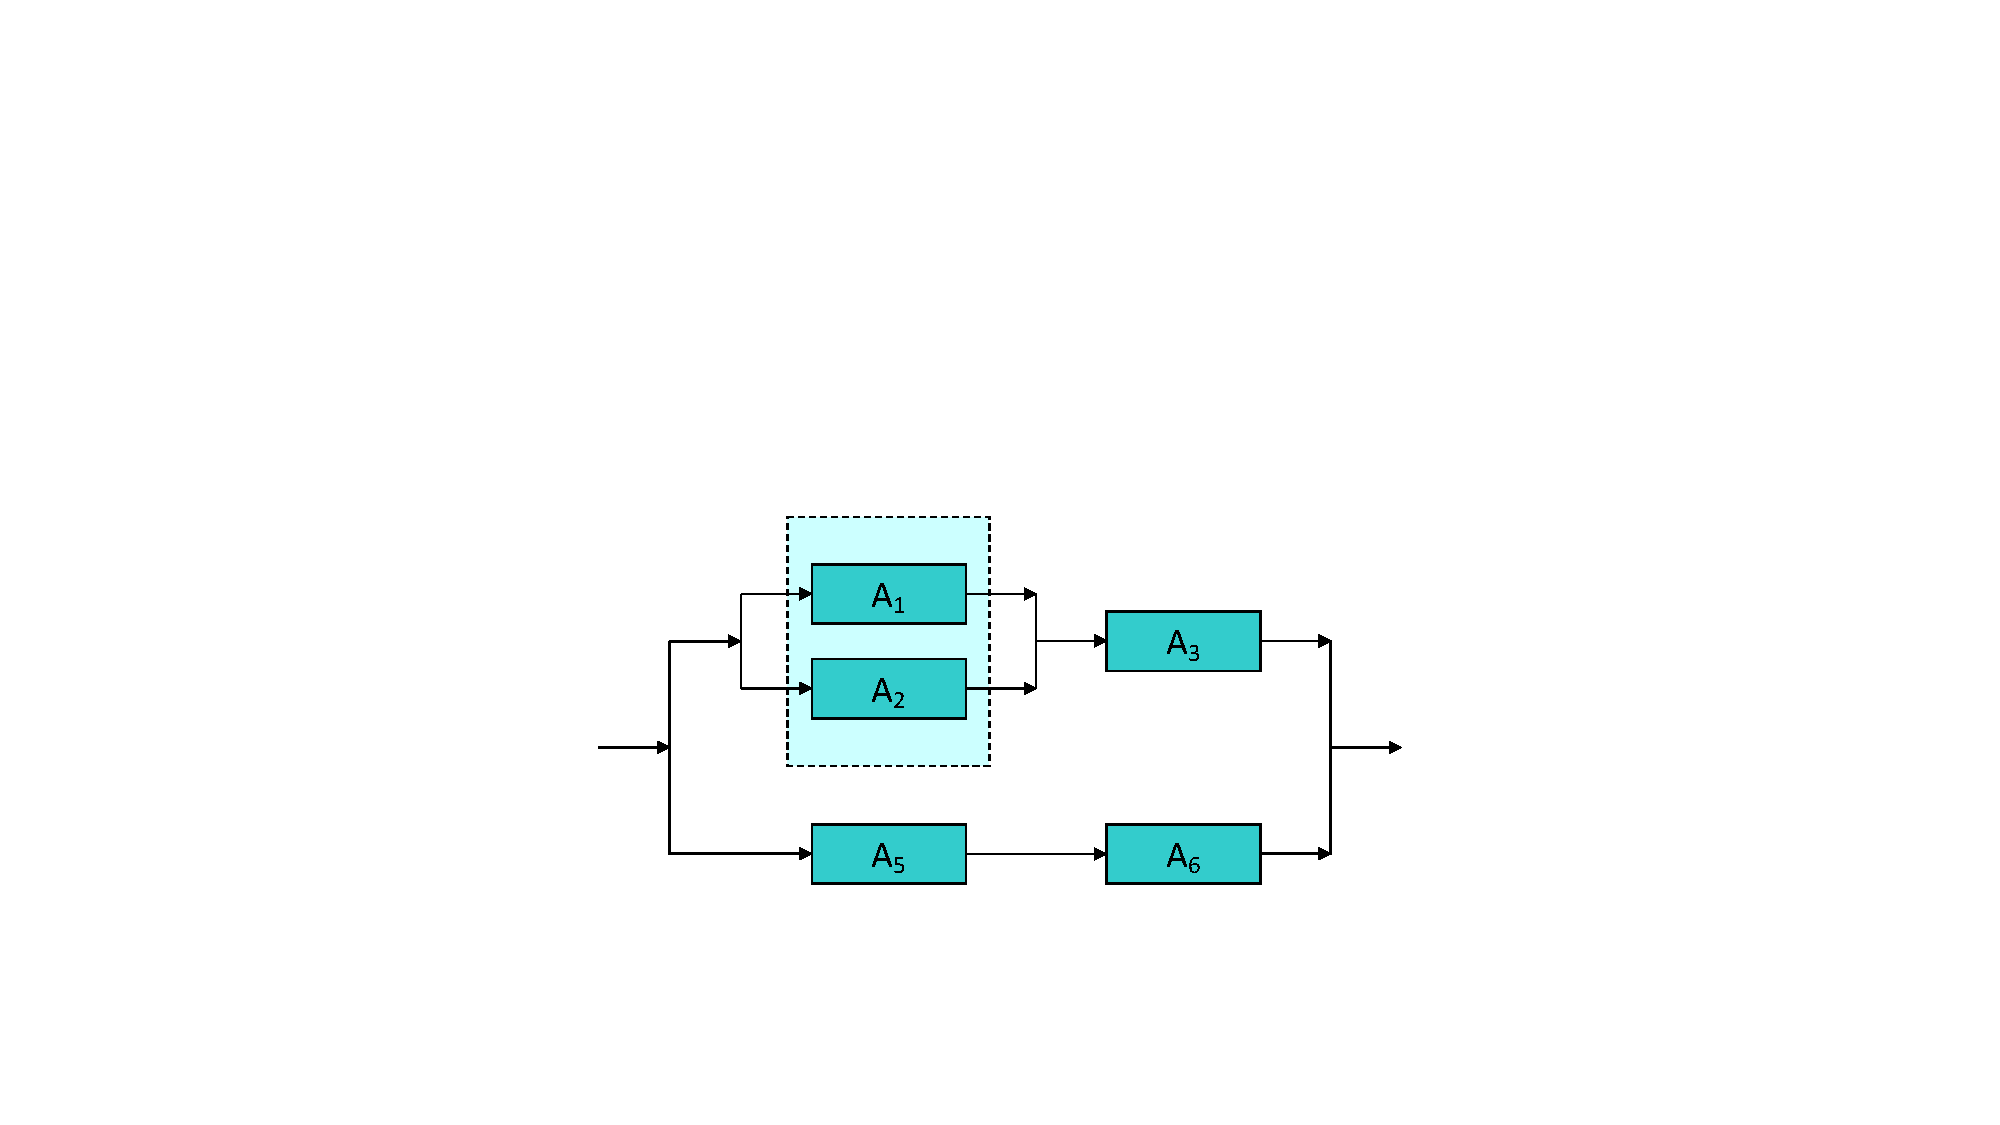
\includegraphics[width=.8\textwidth]{img/availability-in-parallel-1.pdf}
        \end{center}

        \item $A_{8} = A_{7}A_{3}$
        \begin{center}
            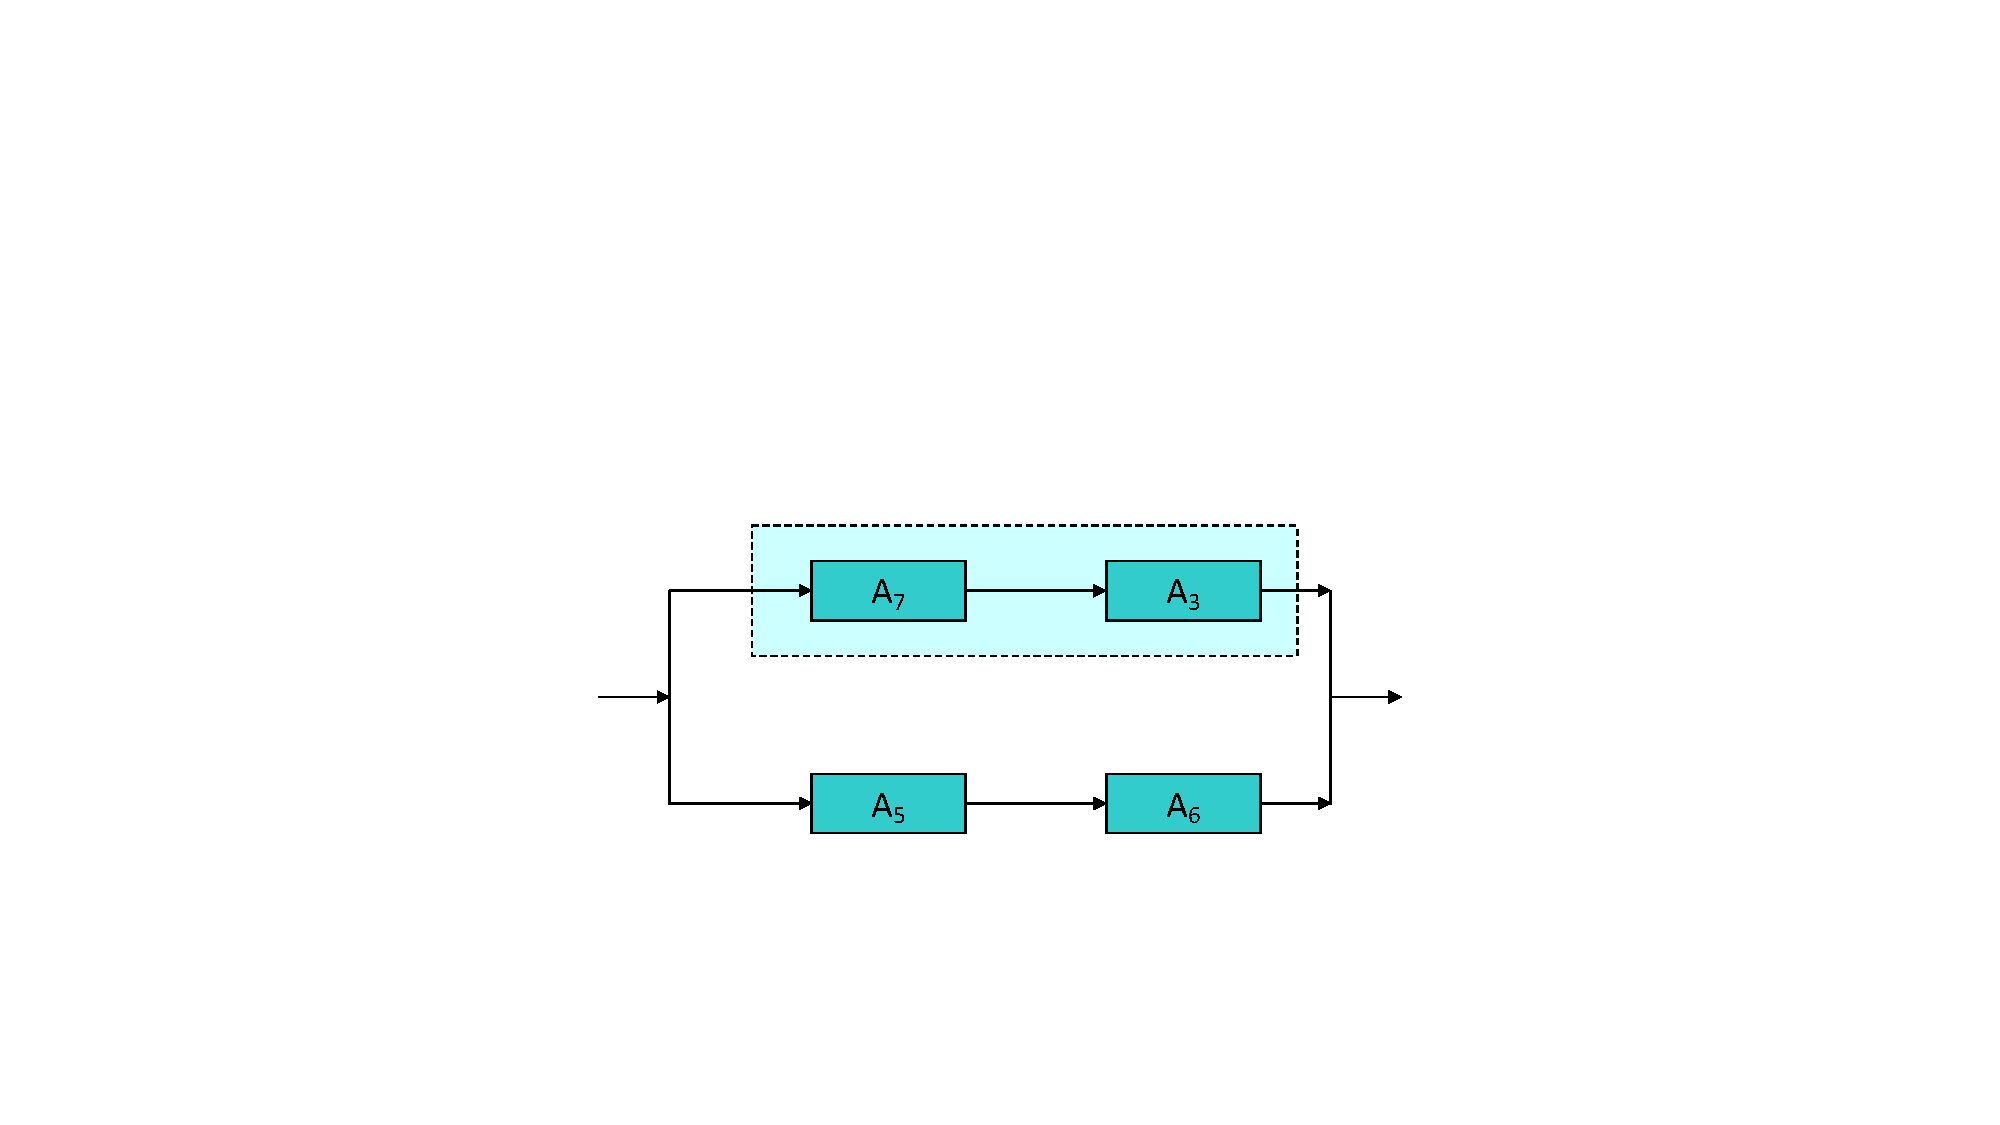
\includegraphics[width=.8\textwidth]{img/availability-in-parallel-2.pdf}
        \end{center}

        \item $A_{9} = A_{5}A_{6}$
        \begin{center}
            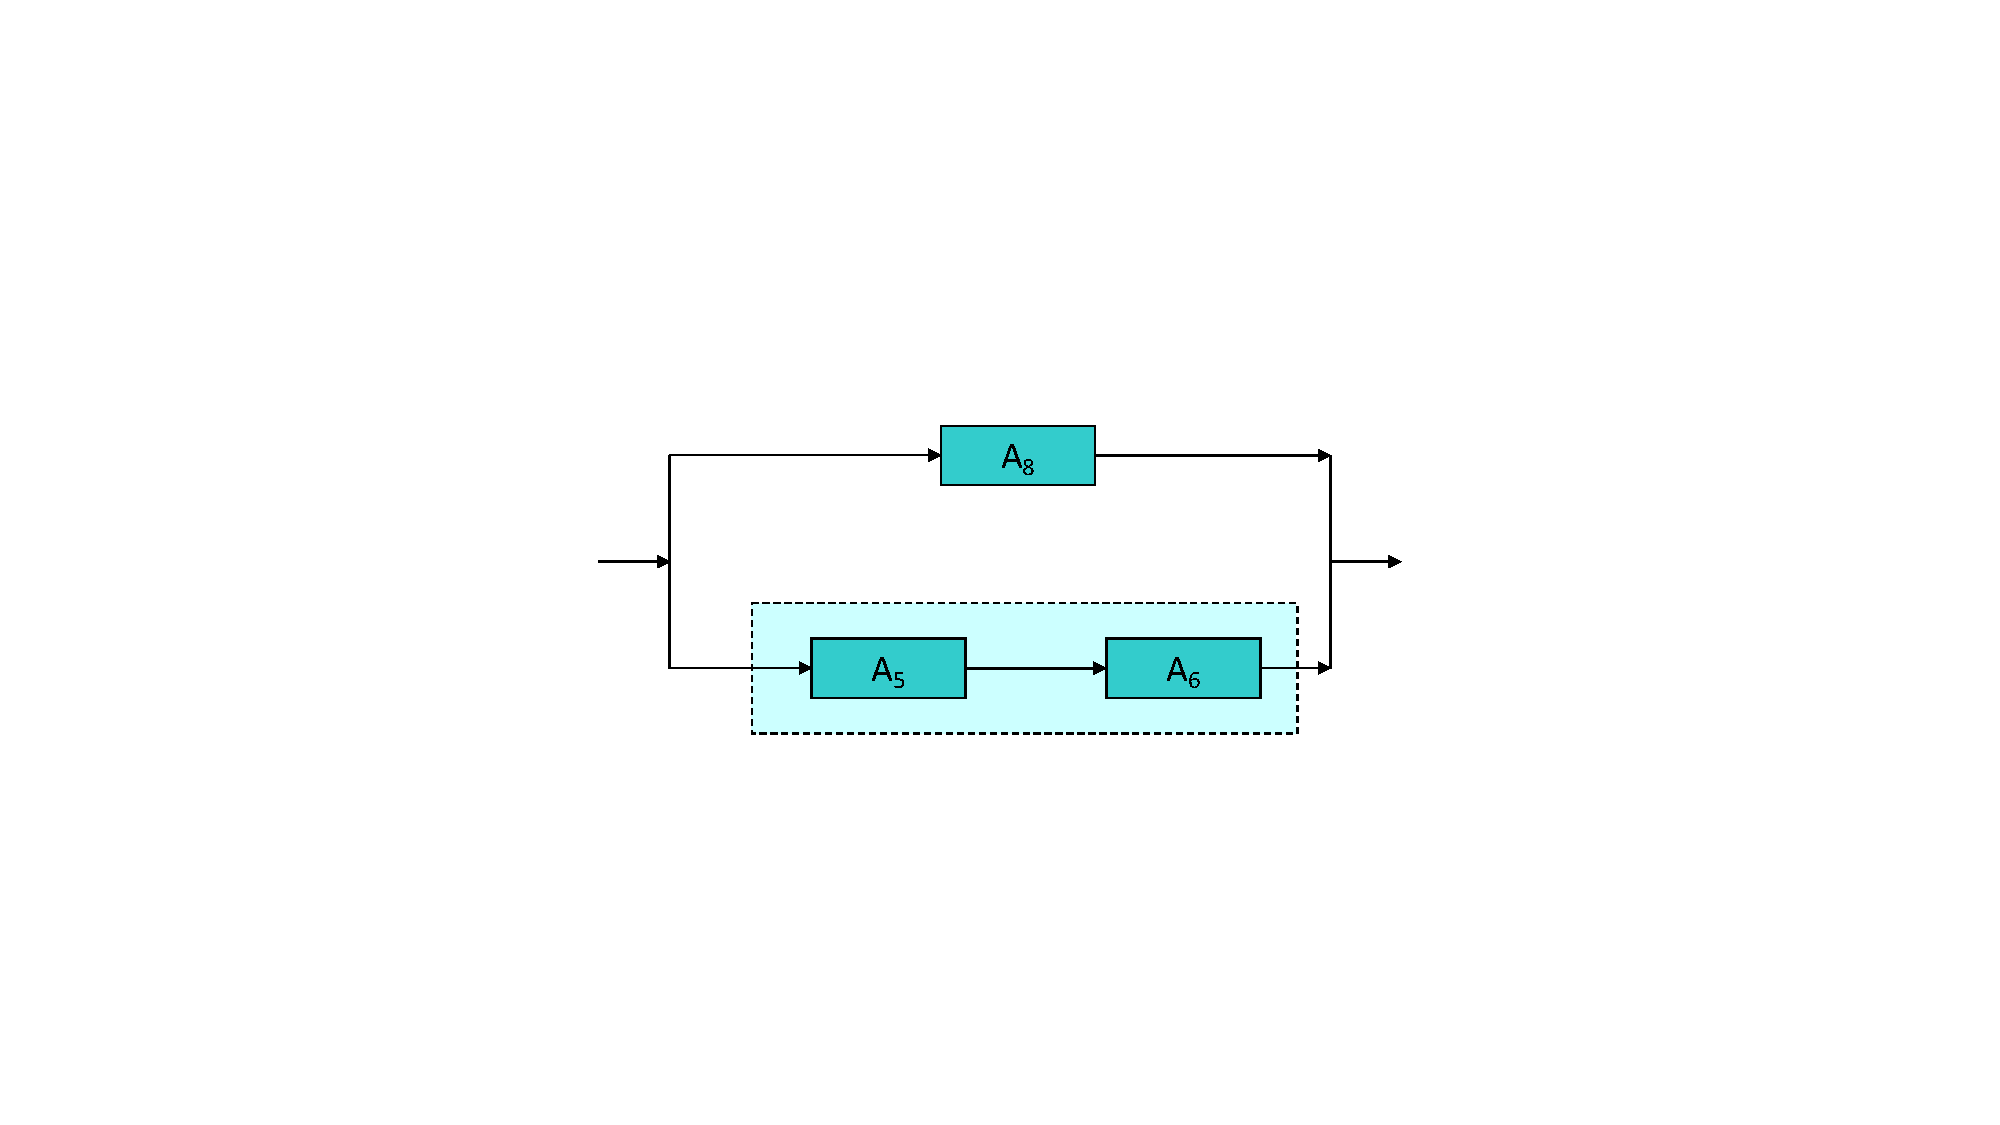
\includegraphics[width=.8\textwidth]{img/availability-in-parallel-3.pdf}
        \end{center}
        
        \item $A = 1 - \left(1-A_{8}\right)\left(1-A_{9}\right)$
        \begin{center}
            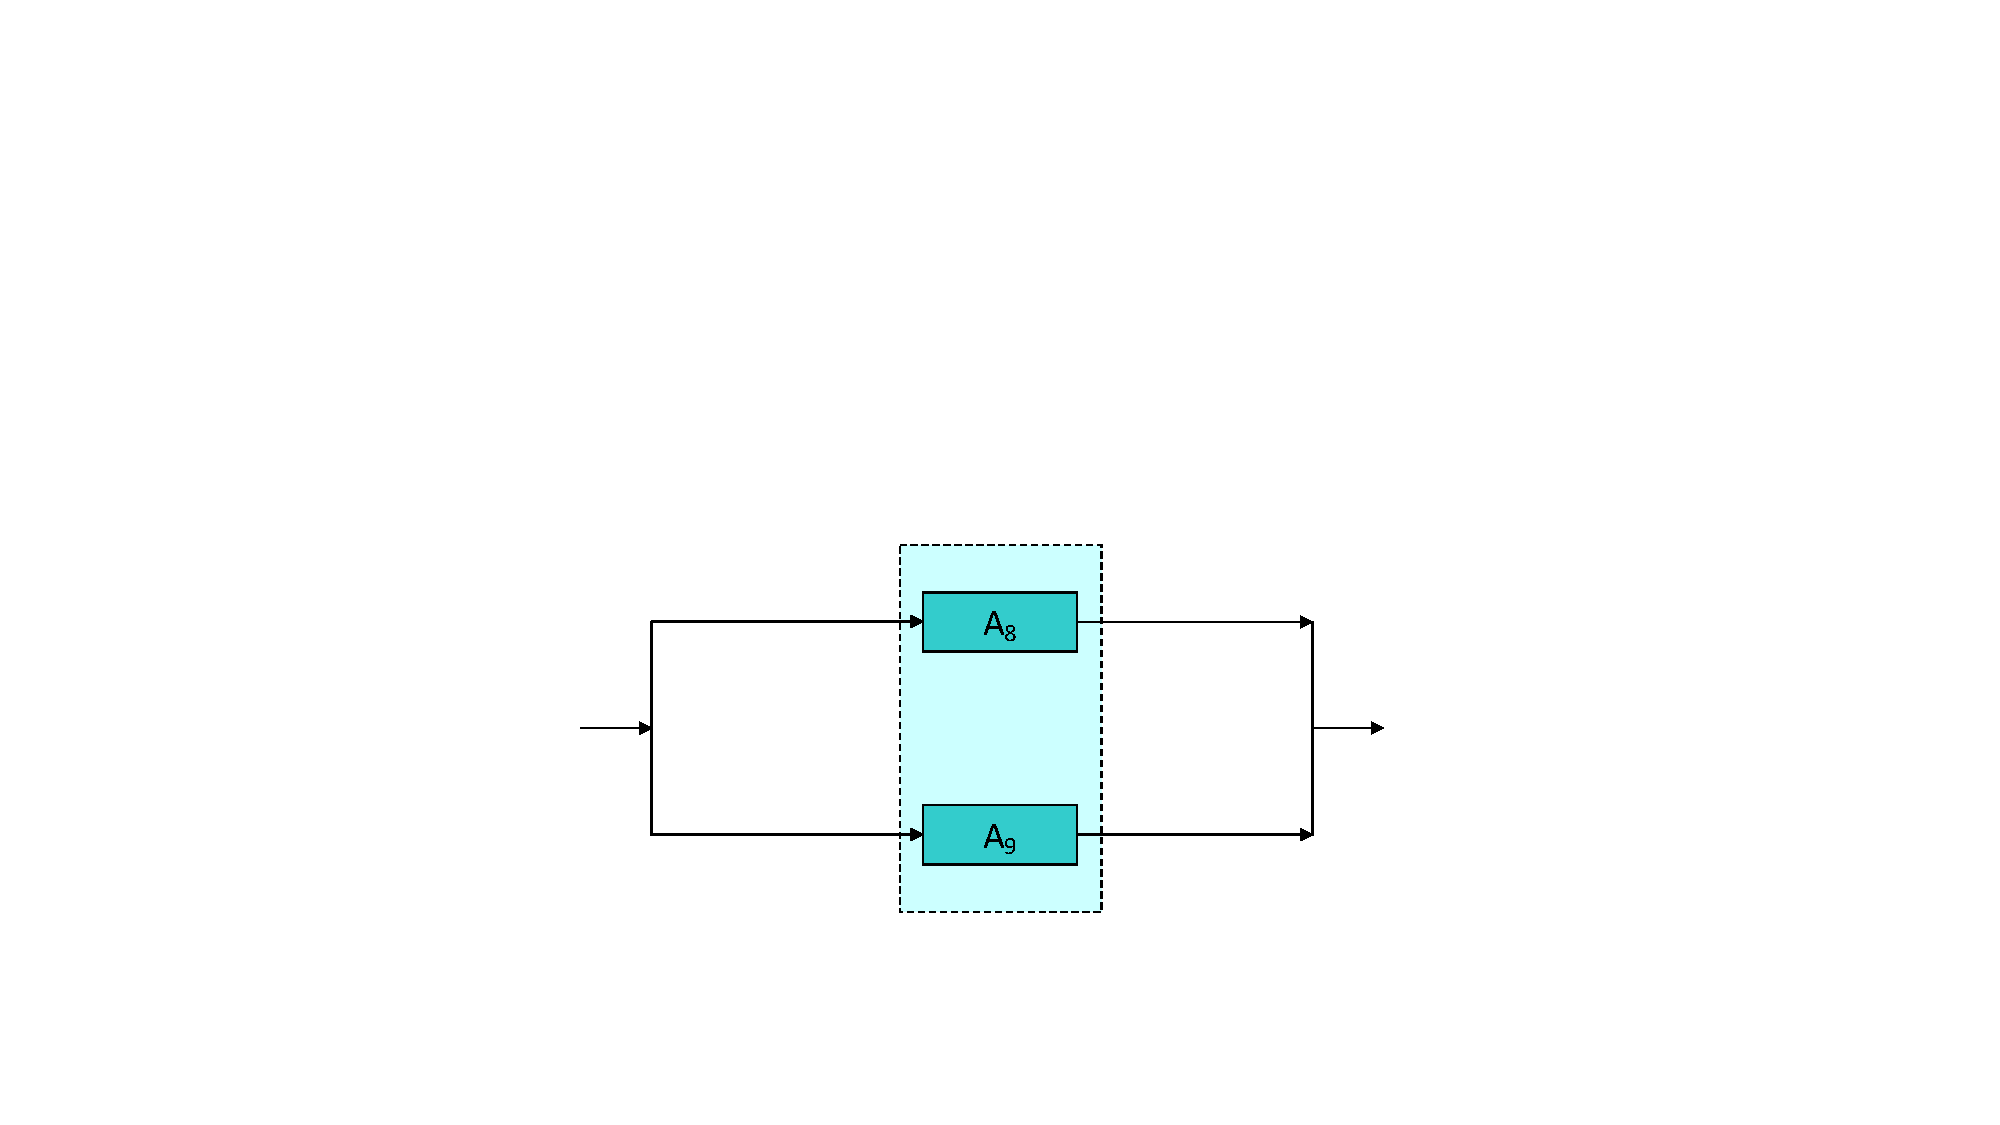
\includegraphics[width=.8\textwidth]{img/availability-in-parallel-4.pdf}
        \end{center}
    \end{itemize}
\end{examplebox}

\newpage

\begin{flushleft}
    \textcolor{Red2}{\faIcon{bookmark} \textbf{Tactics for Availability}}
\end{flushleft}
As we explained in the past pages, Availability is crucial, but it's also fundamental to use intelligent \textbf{tactics to improve the quality of the attributes}.

\begin{definitionbox}
    The \definition{Tactic}s are design decisions that influence the control of one or more quality attributes.
\end{definitionbox}

\noindent
Some well-known tactics are:
\begin{itemize}
    \item \textbf{Replication}
    \item \textbf{Forward error recovery}
    \item \textbf{Circuit breaker}
\end{itemize}

\begin{flushleft}\label{Replication approaches}
    \textcolor{Red2}{\faIcon{book} \textbf{Replication approaches}}
\end{flushleft}
The \definition{Replication} is very simple to manage in the case of stateless components. The approaches are different:
\begin{enumerate}
    \item \definition{Hot spare}: One component leads, and another is always ready to take over.
    
    In the following example, \texttt{C1} leads, \texttt{C2} is always ready to take over.
    \begin{figure}[!htp]
        \centering
        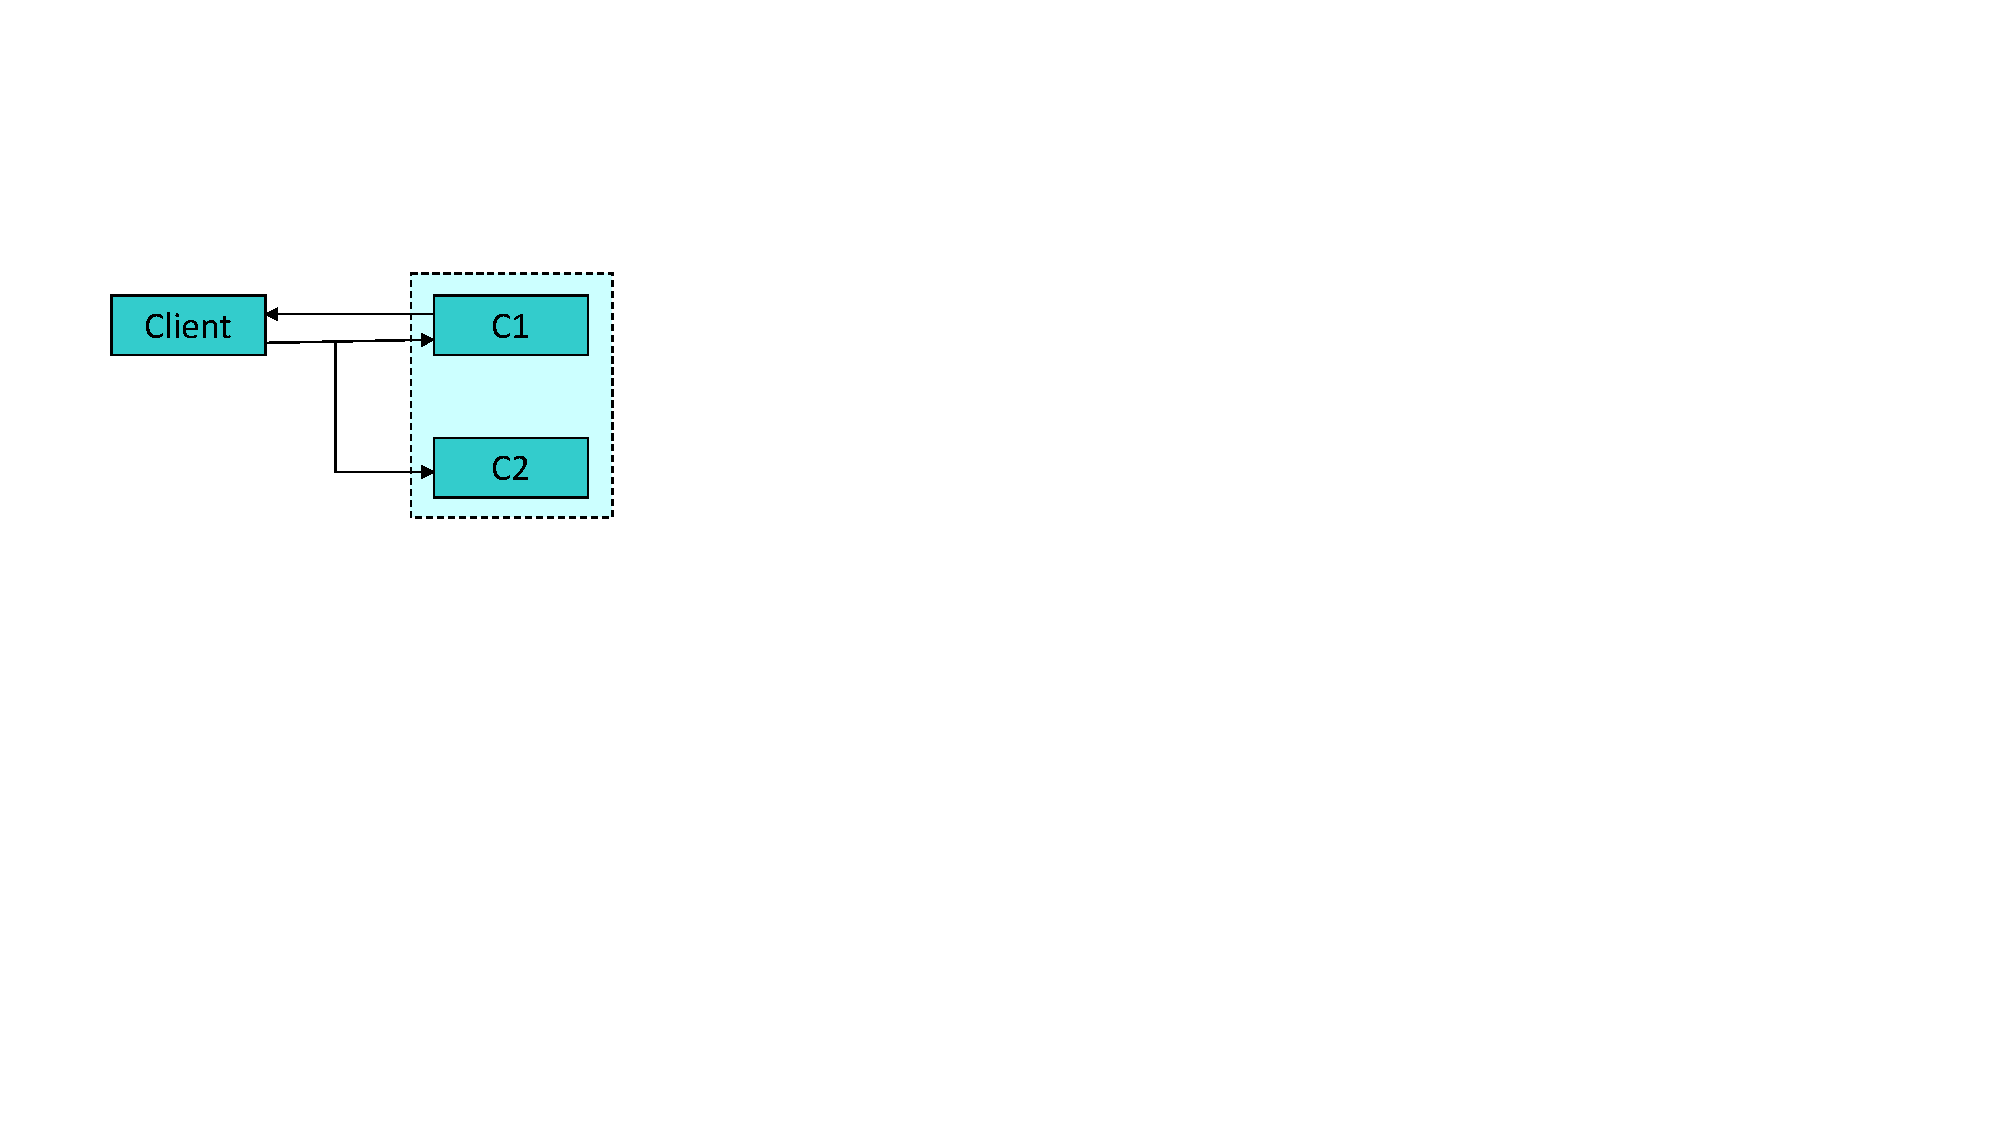
\includegraphics[width=.5\textwidth]{img/replication-1.pdf}
    \end{figure}


    \item \definition{Warm spare}: One component leads and periodically updates another component. If the primary component fails, the second component takes time to update itself fully.
    
    In the following example, \texttt{C1} leads and periodically updates \texttt{C2}. If \texttt{C1} fails, some time might be needed to fully update \texttt{C2}.
    \begin{figure}[!htp]
        \centering
        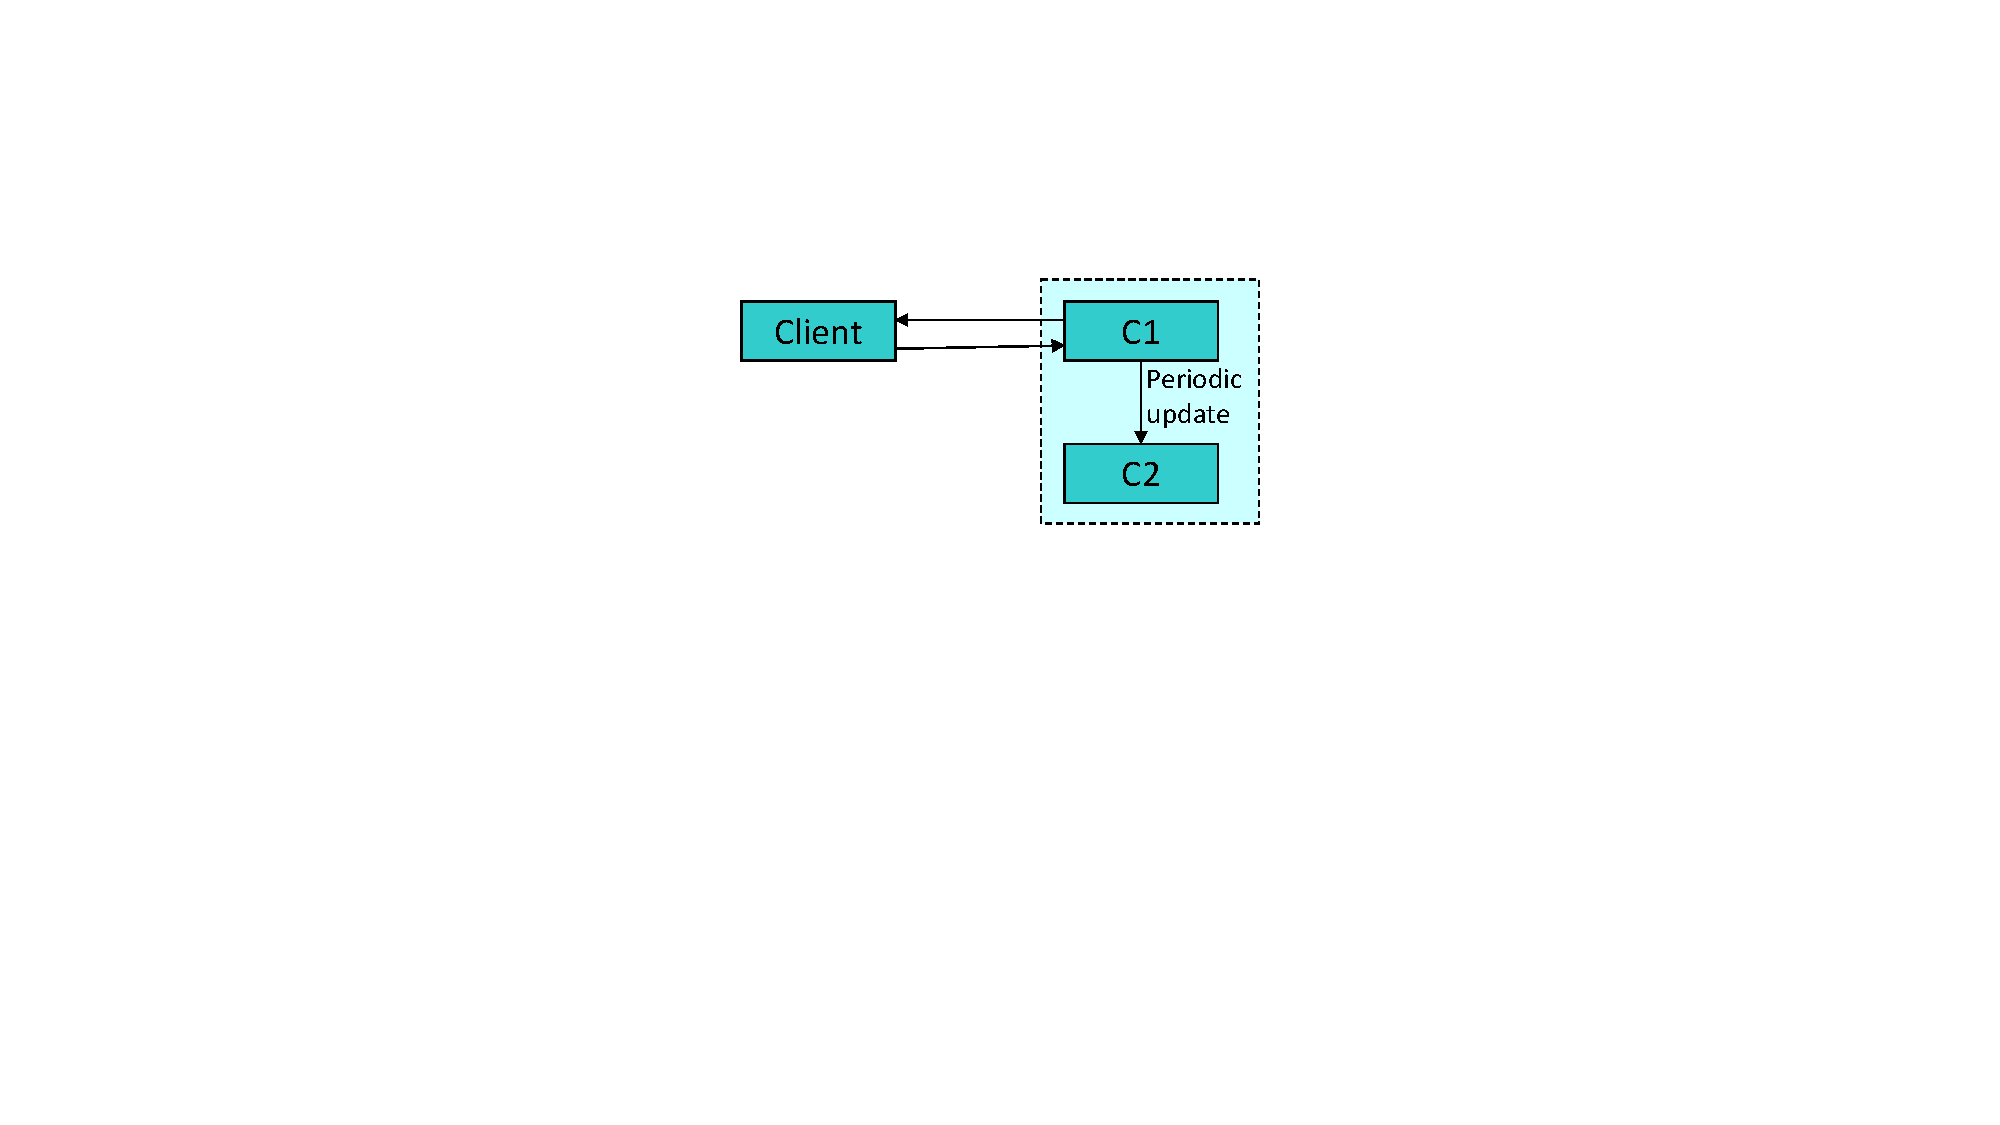
\includegraphics[width=.5\textwidth]{img/replication-2.pdf}
    \end{figure}

    \newpage

    \item \definition{Cold spare}: A second component is dormant, started, and updated only if required.

    In the following example, \texttt{C2} is dormant, started, and updated only if required.
    \begin{figure}[!htp]
        \centering
        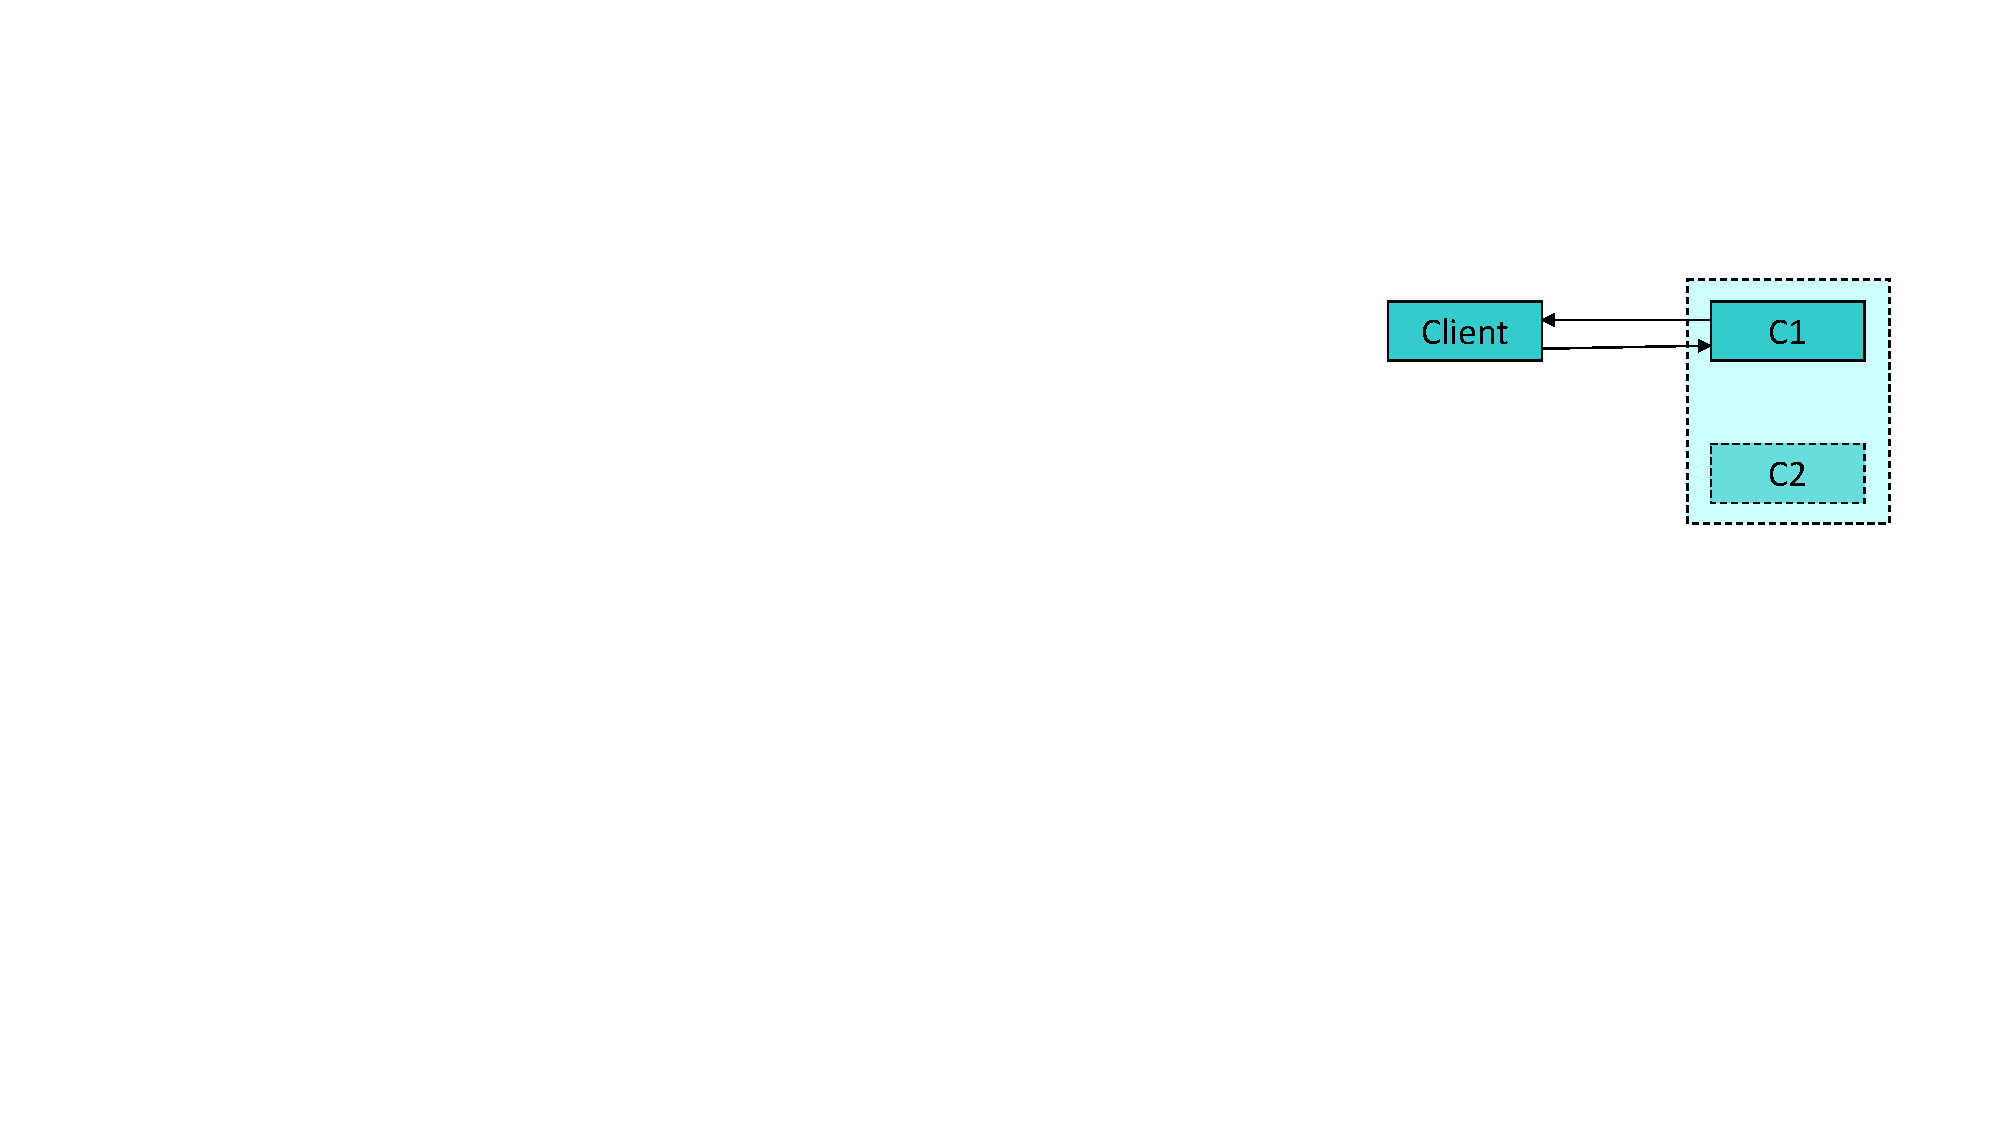
\includegraphics[width=.5\textwidth]{img/replication-3.pdf}
    \end{figure}


    \item \definition{Triple modular redundancy}: Three components are always active, and the result is the one produced by the majority. \textbf{This is good when reliability is also important}.
    
    In the following example, \texttt{C1}, \texttt{C2}, and \texttt{C3} are all active. The result is the one produced by the majority.
    \begin{figure}[!htp]
        \centering
        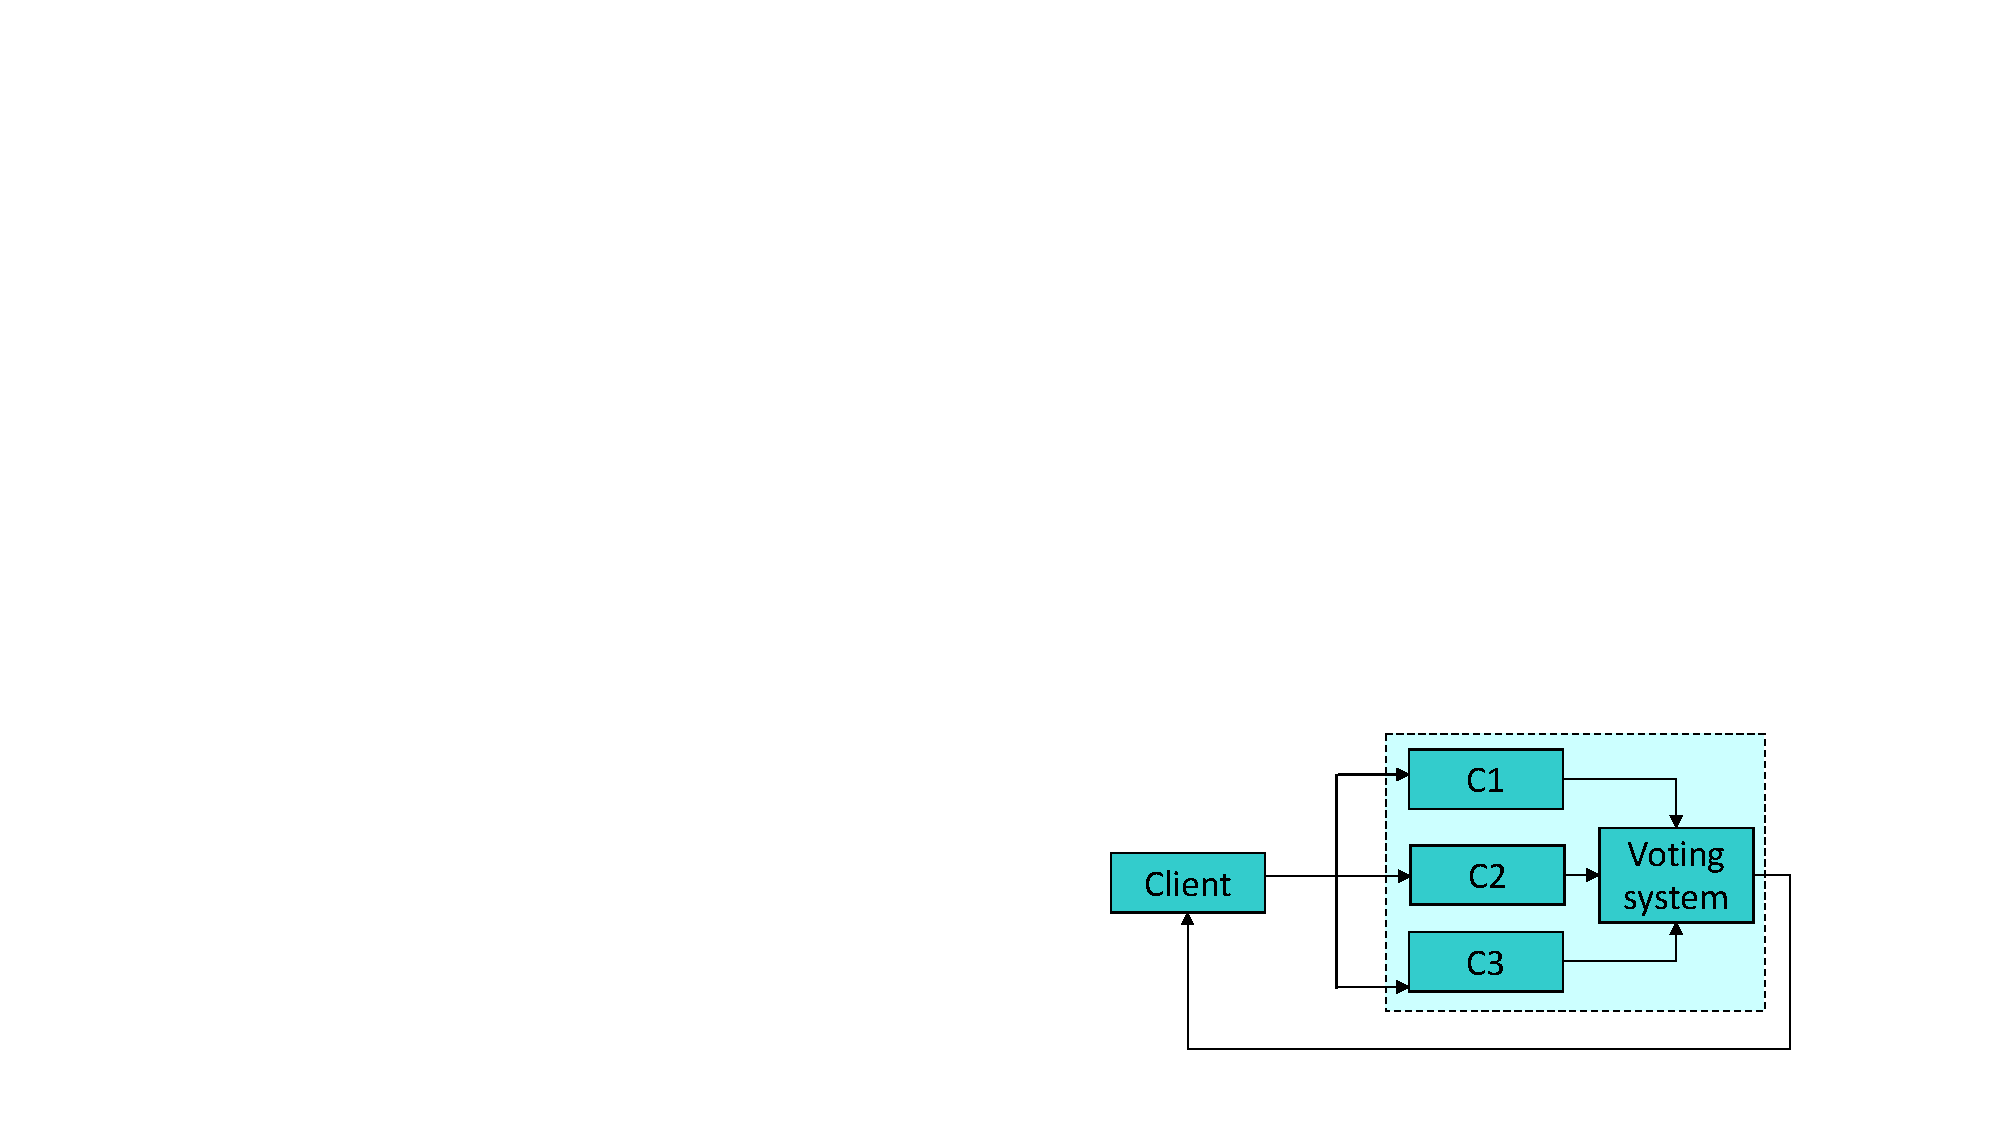
\includegraphics[width=.5\textwidth]{img/replication-4.pdf}
    \end{figure}
\end{enumerate}

\begin{flushleft}
    \textcolor{Red2}{\faIcon{book} \textbf{Forward error recovery}}
\end{flushleft}
\definition{Forward Error Recovery} is a tactic in which a recovery mechanism moves the failed component to a degraded state. In a degraded state, a component continues to be available even if it is not fully functional. Here is an example:

\begin{figure}[!htp]
    \centering
    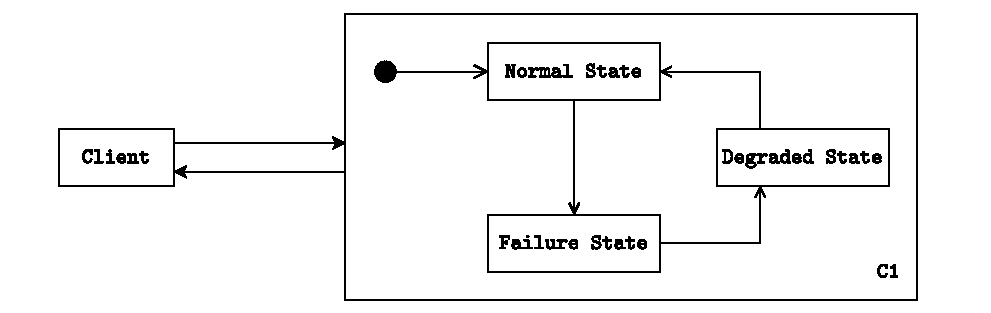
\includegraphics[width=\textwidth]{img/forward-error-recovery-1.pdf}
\end{figure}

\newpage

\begin{flushleft}
    \textcolor{Red2}{\faIcon{book} \textbf{Circuit breaker}}
\end{flushleft}
The \definition{Circuit Breaker (CB)} tactic is a client-side resiliency pattern. The CB acts as a proxy for a remote component:
\begin{enumerate}
    \item A component is called;
    \item The CB monitors the call.
\end{enumerate}
But note that there should be possible failures:
\begin{itemize}
    \item CB receives an error;
    \item The call takes \dquotes{too long} (CB kills the call).
\end{itemize}
If there are too many failures, the circuit breaker inhibits future calls by moving to the open state.

\begin{figure}[!htp]
    \centering
    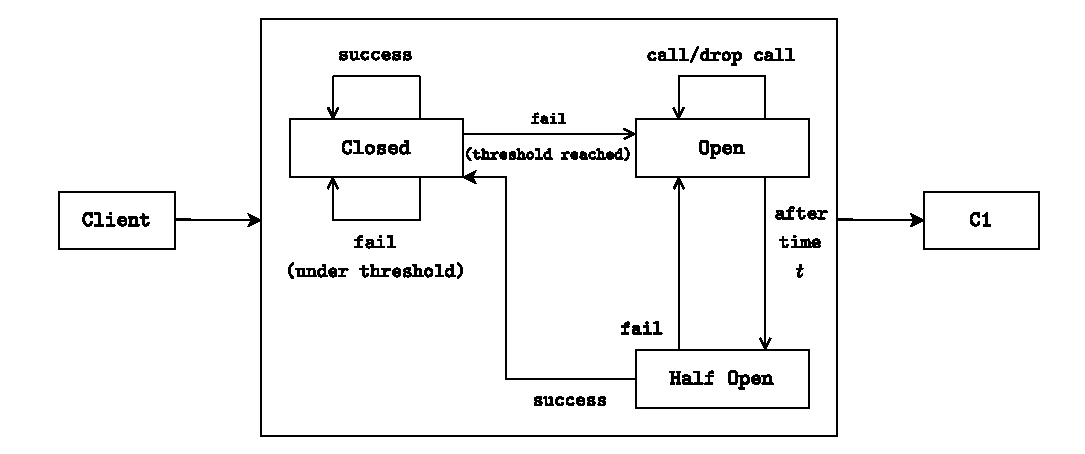
\includegraphics[width=\textwidth]{img/circuit-breaker-1.pdf}
\end{figure}